% This file was converted to LaTeX by Writer2LaTeX ver. 1.6.1
% see http://writer2latex.sourceforge.net for more info
\documentclass[11pt,parskip=half,a4paper]{scrartcl}
\usepackage[latin9]{inputenc}
\usepackage{amsmath}
\usepackage{amssymb,amsfonts,textcomp}
\usepackage[T1]{fontenc}
\usepackage[english]{babel}
\usepackage{multicol}
\usepackage{array}
\usepackage{hhline}
\usepackage{graphicx}
\usepackage{pslatex}
\usepackage{helvet}
\usepackage{listings}

% Text styles
\newcommand\textstyleStrongEmphasis[1]{\textbf{#1}}
\newcommand\textstyleSourceText[1]{\texttt{#1}}
\newcommand\textstyleEmphasis[1]{\textit{#1}}

\lstset{numbers=left, numberstyle=\tiny, numbersep=4pt, breaklines=true, frame=single, showstringspaces=false, basicstyle=\scriptsize}
\include{lua.def}
\usepackage[pdftitle={HeliTrim Manual},pdfstartview={FitH},colorlinks=true]{hyperref}
\pdfcompresslevel=9
\pdfimageresolution=72

\usepackage{color}
\definecolor{hellgrau}{gray}{0.85}
\definecolor{dunkelgrau}{gray}{0.55}

\newcommand{\hinweis}[2]{%
\phantomsection\addcontentsline{toc}{section}{#1}
\begin{center}
\fcolorbox{dunkelgrau}{hellgrau}{\parbox{14cm}{\textbf{#1}#2}}
\end{center}
}

\newcounter{aufg}
\newcommand{\xsb}{XSquawkBox}
\newcommand{\punkte}[1]{\marginpar{\fcolorbox{dunkelgrau}{hellgrau}{\parbox{4.5ex}{\sffamily\tiny#1}}}}

\renewcommand{\labelenumi}{\alph{enumi})}

\newcommand{\aufgabe}{\stepcounter{aufg}\vspace{0.75cm}\pagebreak[3]{\phantomsection\addcontentsline{toc}{section}{Aufgabe~\arabic{aufg}}\Large\sffamily Aufgabe~\arabic{aufg}}}
\renewcommand{\labelenumi}{\alph{enumi})}

\usepackage{fancyhdr}
\usepackage{lastpage}
\pagestyle{fancy}

\setlength{\headheight}{2cm}
\cfoot{\footnotesize Page \thepage\ of \pageref{LastPage}}
\renewcommand{\headrulewidth}{0.4pt}
\renewcommand{\footrulewidth}{0.4pt}

\begin{document}

\title{Xchecklist Reference Manual}
\author{Michal \& Bill}
\date{\today}

\maketitle

\begin{center}
1.34
\end{center}

\vspace{2cm}


\begin{center}
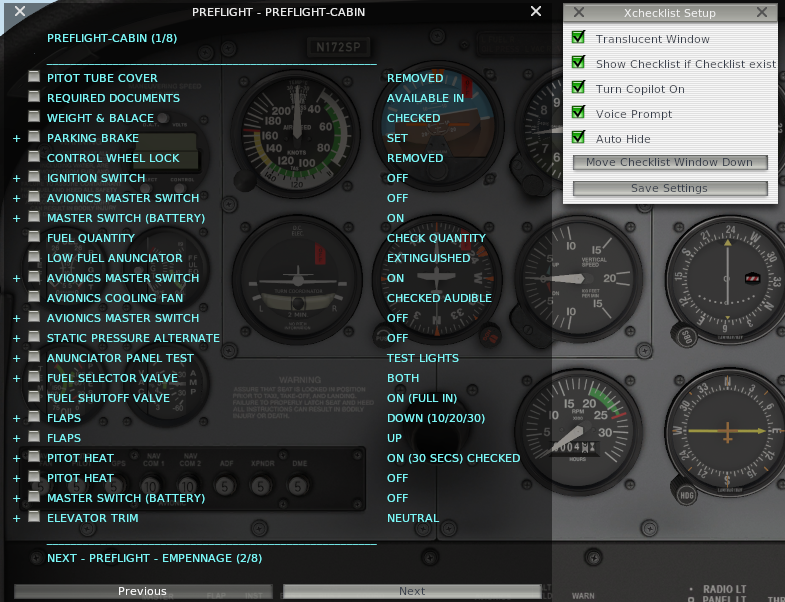
\includegraphics[width=15cm]{TranslucentXchecklist.png}
\end{center}


\thispagestyle{empty}
\newpage
\verb||
\tableofcontents

\newpage
\section{History}

Xchecklist started out as a Linux checklist program to fill a void that was there in fall of 2010. Michal and I worked on it and initially was only in the forums and then it was in the download section. It looks like there is another void as there is no 64 bit checklist program. \newline

In the beginning of August 2013 I contacted Michal and told him I would like to port our Xchecklist to be multi-platform and 32/64 bit. He was on board and now we have a version that does work on all three platforms and is 32/64bit.

\section{Feature List}
 
\begin{itemize}
\item Drop-in replacement for snailpup's checklister plugin
\end{itemize}

\begin{itemize}
\item Win/Mac/Lin 32/64 bit \& 9.70 compatible
\end{itemize}

\begin{itemize}
\item Features speaking {\textquotedbl}copilot{\textquotedbl} saying checklist items for you
\end{itemize}

\begin{itemize}
\item Features native speech for each platform to allow more options \ \ \ 
\end{itemize}

\begin{itemize}
\item Copilot may also check some actions for you as you perform them
\end{itemize}

\begin{itemize}
\item Actions (Check, Prev, Next, Hide, Reload) can be mapped to key/joystick button of choice
\end{itemize}

\begin{itemize}
\item Enforces strictly sequential checklist flow
\end{itemize}

\begin{itemize}
\item Allow colored text for some items in a checklist
\end{itemize}

\newpage
\section{Installation Instructions}

Unpack the archive and place the folder Xchecklist to '.../Resources/plugins' then fire up XPlane and if the plane you fly has a checklist, you should see it.. \newline

If you are using a version previous to 1.34 please delete the ../Resources/plugins/Xchecklist folder and install the new one as the folder structure has changed with this version. \newline 

The checklist file is called clist.txt and should be put in the aircraft folder which is the same place the *.acf file resides. \newline

You may also have a checklist file named aircraftname\_clist.txt which will be searched for first then it will search for clist.txt. The default Cessna would be Cessna\_172SP\_clist.txt. This allows you to have multiple aircraft in one folder like a float and a wheeled version. \newline

Also in the archive is a folder called Xchecklist/Checker \ that has test programs for your platform and bitsize. \newline

Paths are bgood/xchecklist/check\_item, \ \ bgood/xchecklist/next\_checklist, \ bgood/xchecklist/prev\_checklist, \ \ bgood/xchecklist/hide\_checklist and bgood/xchecklist/reload\_checklist. \newline

If you have any ideas, comments or bug reports, don't hesitate and let us know... \newline

Kind regards, \newline

Michal \& Bill \newline

\newpage
\section{Xchecklist Setup}

\begin{center}
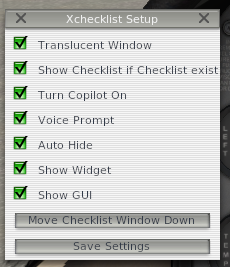
\includegraphics[width=6cm, height=5cm]{XchecklistSetup.png}
\end{center}


The {\textquotedbl}Xchecklist Setup{\textquotedbl} dialog box will be explained first and can be found by clicking on the Plugins menu item and selecting Xchecklist from the drop down list. 

\textbf{Translucent Window} when checked makes the checklist translucent.

Unchecked the checklist is solid. \newline

\textbf{Show Checklist if Checklist exist} when checked if there is a clist.txt for the aircraft loaded it will 
display the checklist. 

Unchecked it will not display the checklist. \newline

\textbf{Turn Copilot On} when checked will automatically check in order items that have data refs in the 
clist.txt. These items are marked with a + sign in front of the check box. 

Unchecked you have to check each item yourself. \newline

\textbf{Voice Prompt} when checked will speak a prompt for the upcoming item.

Unchecked it is quiet. \newline

\textbf{Auto Hide} when checked will automatically hide the checklist after it is complete and a small delay. 

Unchecked it will not hide. \newline

\newpage

\textbf{Show Widget} when checked shows the older widget checklist. \newline

\textbf{Show GUI} when checked shows the new GUI checklist that can be scaled and popped to a second display.
It is also the checklist widow type that is used in VR but in VR it has a transparent background. \newline

\textbf{Move Checklist Window Down} will move the checklist window down so you can grab it with the mouse if it is up under the top menu bar. \newline

\textbf{Save Settings} will save your settings including the window position of the checklist in a preference file. Before saving the window position it will make sure that what is saved is within the current screen. \ As a side benefit if you changed screen resolution and part of the checklist is outside the current screen pressing this button will put it back inside the screen.

\newpage
\section{X-Plane 10 Joystick buttons setup}

Joystick buttons are setup using Buttons : Adv pane in the Joystick \& Equipment window, that is accessible through Settings / Joystick, Keys \& Equipment menu.

\begin{center}
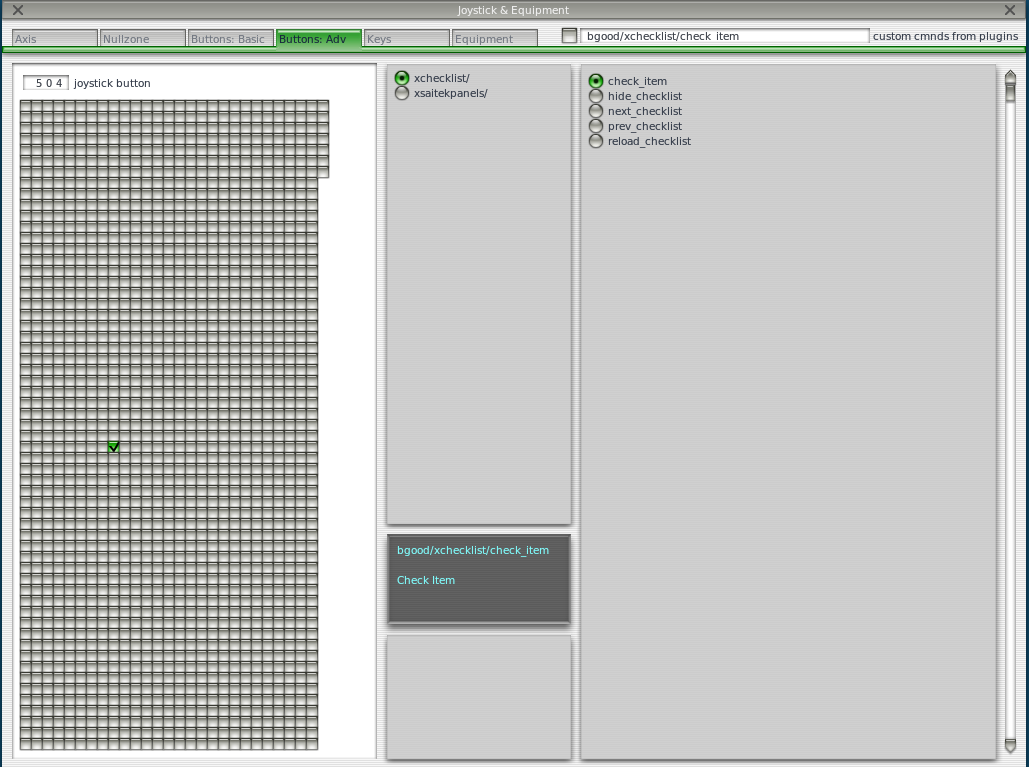
\includegraphics[width=17cm]{XchecklistUserManual-img001.png}
\end{center}

Please note the four items in the right box - these are the four actions, that allow you to control the Xchecklist. \newline

Now just press the desired joystick button, in the upper middle box select xchecklist/ and in the right 
box select the appropriate action. \newline

Repeat those steps and when done, just close the window and the new bindings should be active. 
First item is 'check\_item' that checks a item. 

\newpage
Next item is 'next\_checklist' that moves to the next page of the checklist. If the checklist is hidden it 
will also un hide it without moving to the next page. 

Next item is 'prev\_checklist' that moves to the prev page of the checklist.

Next item is 'hide\_checklist' as it says hides the checklist.

Reload item is 'reload\_checklist' as it says reloads the checklist.

\newpage
\section{X-Plane 10 Keystrokes setup}
Keystrokes are setup using Keys pane in the Joystick \& Equipment window, that is accessible through 
Settings / Joystick, Keys \& Equipment menu.

\begin{center}
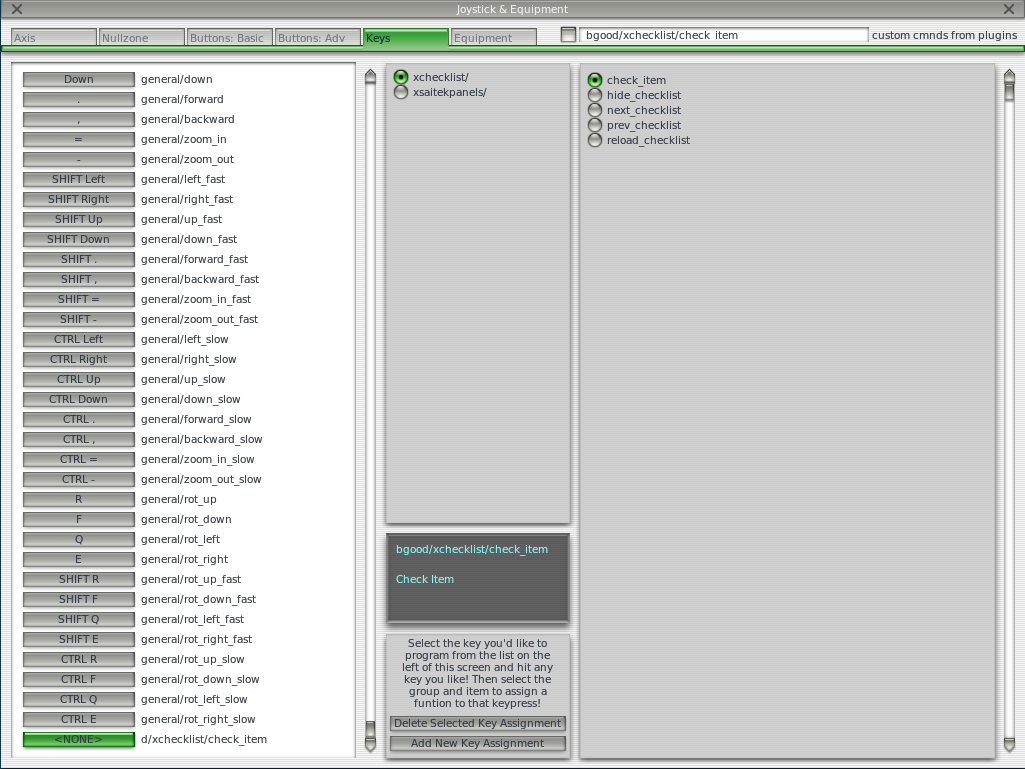
\includegraphics[width=17cm]{XchecklistUserManual-img002.png}
\end{center}

Please note the four items in the right box - these are the four actions, that allow you to control the 
Xchecklist. 

Now just press the desired keystroke, in the left box select xchecklist/ and in the right box select the 
appropriate action. 

Repeat those steps and when done, just close the window and the new bindings should be active. 

First item is 'check\_item' that checks a item. 

Next item is 'next\_checklist' that moves to the next page of the checklist. If the checklist is hidden it 
will also un hide it without moving to the next page. 

Next item is 'prev\_checklist' that moves to the next page of the checklist.

Next item is 'hide\_checklist' as it says hides the checklist.

Last item is 'reload\_checklist' as it says reloads the checklist.

\newpage
\section{X-Plane 11 Joystick buttons setup}

Joystick buttons are setup using Settings dialog window which can be accessed through the Settings button on the first screen. Use the Joystick menu.

\begin{center}
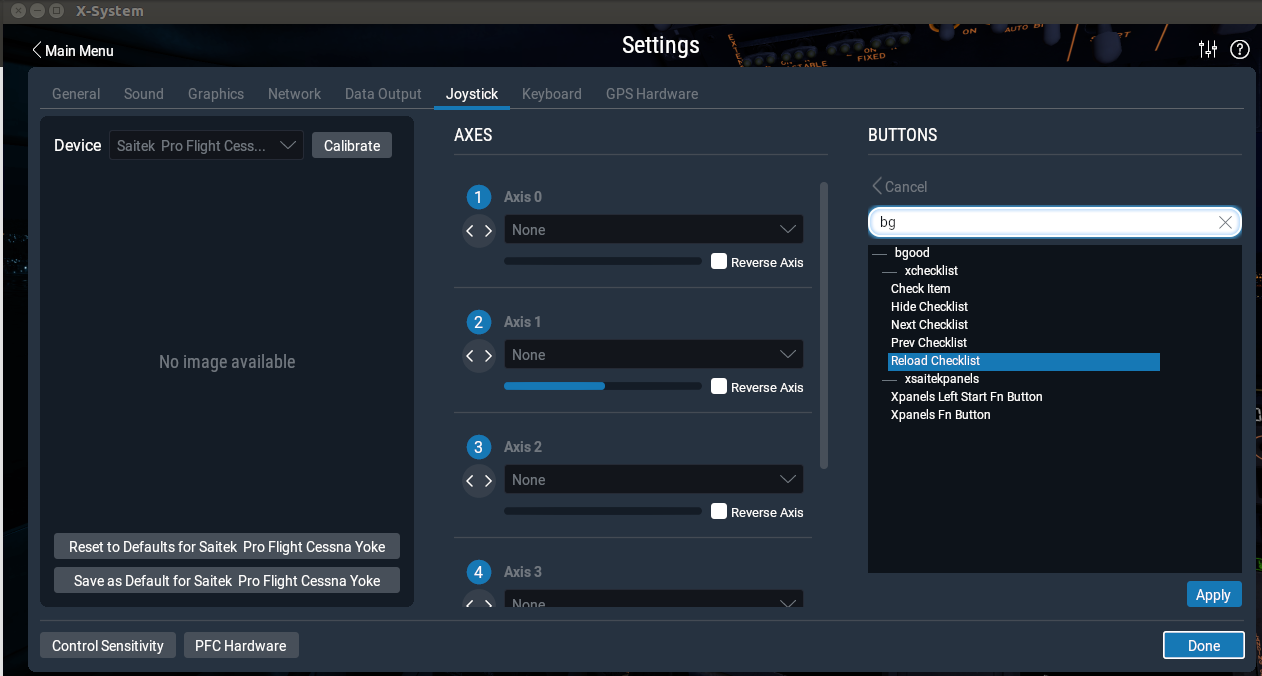
\includegraphics[width=17cm]{XchecklistUserManual-img003.png}
\end{center}

Please note the four items in the right box - these are the four actions, that allow you to control the 
Xchecklist. 

Now just press the desired joystick button, on the right hand side you will see the button hi light. Click on the Edit button and type bg in the search box. Select the action you want to map and then click on the Apply button. Repeat these steps for the remaining actions. When you are done press the Done button.

First item is 'check\_item' that checks a item. 

Next item is 'next\_checklist' that moves to the next page of the checklist. If the checklist is hidden it 
will also un hide it without moving to the next page. 

Next item is 'prev\_checklist' that moves to the prev page of the checklist.

Next item is 'hide\_checklist' as it says hides the checklist.

Reload item is 'reload\_checklist' as it says reloads the checklist.


\newpage
\section{X-Plane 11 Keystrokes setup}

Keystrokes are setup using Settings dialog window which can be accessed through the Settings button on the first screen.Use the Keyboard menu.

\begin{center}
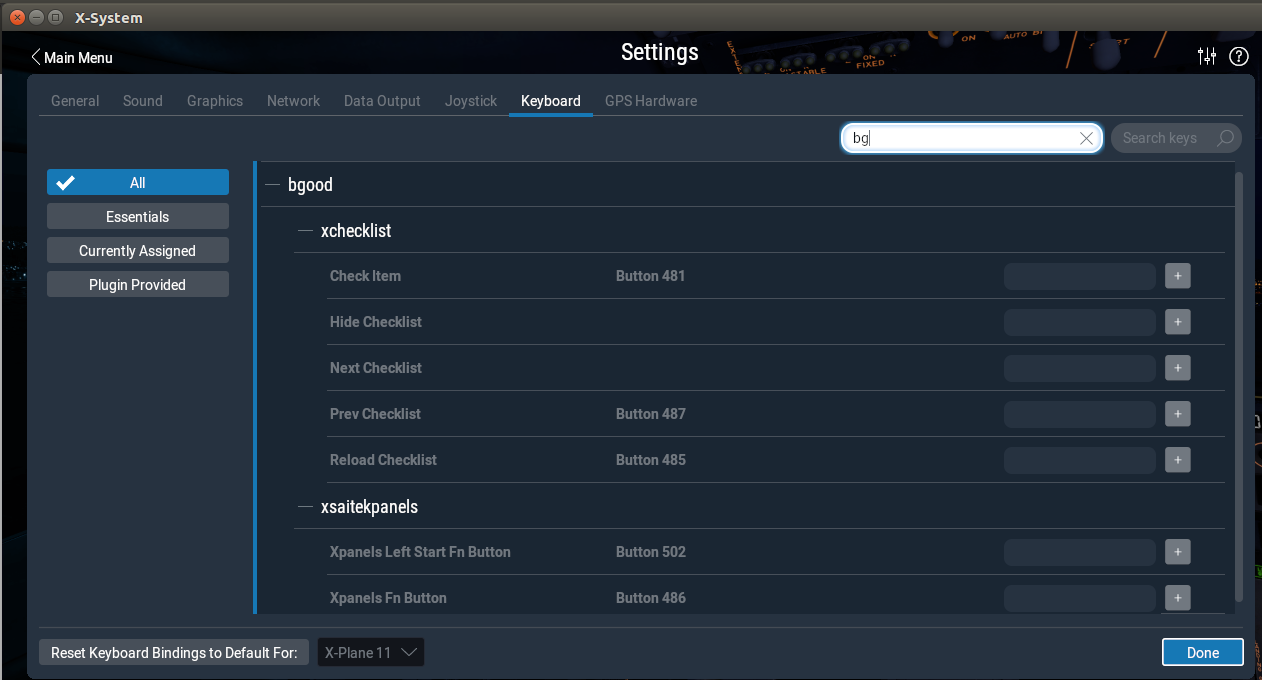
\includegraphics[width=17cm]{XchecklistUserManual-img004.png}
\end{center}

After typing bg in the search box you should see the items you can map to Xchecklist.

Now just click on the gray box to the left of the + sign of the item you want to map. When you do this the gray box will turn white and will say ``Record keystroke(s)'' . Record your keystrokes and the box will turn gray again with your recorded keystrokes in the gray box. You will now also see a + sign and a -- \ sign.

Repeat those steps and when done, press the done button. 

First item is 'check\_item' that checks a item. 

Next item is 'next\_checklist' that moves to the next page of the checklist. If the checklist is hidden it 
will also un hide it without moving to the next page. 

Next item is 'prev\_checklist' that moves to the next page of the checklist.

Next item is 'hide\_checklist' as it says hides the checklist.

Last item is 'reload\_checklist' as it says reloads the checklist.

\newpage
\section{Checklist files}

When the X-Plane loads a plane, Xchecklist looks to the airplane's directory and tries to load the acf specific
checklist first (acfName\_clist.txt), and if not found, the generic clist.txt is loaded.


\section{Checklist file structure}

The checklist file contains series of checklists for the given aircraft.

Each checklist starts with the \textstyleStrongEmphasis{sw\_checklist}. This statement specifies the title of the checklist, and optionally the name, under which it appears in the XChecklist's menu (when the optional part is missing, the menu item is not created). This way the {\textquotedbl}entry points{\textquotedbl} of multi-page checklists are accessible via menu, without cluttering the menu with the interim pages.

\textstyleSourceText{sw\_checklist:Checklist name}

\ textstyleSourceText{sw\_checklist:Checklist name:Menu name}

The checklist itself can contain several types of statements:

\begin{itemize}
\item \textstyleStrongEmphasis{sw\_item} - normal checklist item - spoken by copilot, checkable both manually and automaticaly 
\item \textstyleStrongEmphasis{sw\_iteminfo} - checklist item, checkable only by fulfilling the condition 
\item \textstyleStrongEmphasis{sw\_itemvoid} - noncheckable checklist item; ignored by copilot 
\item \textstyleStrongEmphasis{sw\_remark} - remarks spoken by copilot (no condition, non-checkable) 
\item \textstyleStrongEmphasis{sw\_show} - when no checklist is displayed and a condition is fulfilled, the checklist pops up 
\item \textstyleStrongEmphasis{sw\_continue} - designates which checklist should come next, when the current one
finishes 
\item \textstyleStrongEmphasis{sw\_rcolsize} - specifies the size of the {\textquotedbl}right column{\textquotedbl} of the checklist 
\end{itemize}
\subsection{sw\_item}
This is the most used checklist item. There are several forms of this item:

\textstyleSourceText{sw\_item:Item text}

\textstyleSourceText{sw\_item:Item text{\textbar}Checked text}

{\ttfamily
\textstyleSourceText{This form displays a checkbox with the {\textquotedbl}Item text{\textquotedbl} caption; if the text contains a colon character,}}

{\ttfamily
\textstyleSourceText{the text following it is displayed on the right side, otherwise the text
{\textquotedbl}CHECK{\textquotedbl} is used.}}

{\ttfamily
\textstyleSourceText{The checkbox must be checked by the pilot.}}

\textstyleSourceText{sw\_item:Item text:dataref expression}

{\ttfamily
\textstyleSourceText{This form allows the {\textquotedbl}copilot{\textquotedbl} check the item for you based on the dataref expression}}

\subsection[Dataref expressions]{Dataref expressions}
Dataref expressions allows the {\textquotedbl}copilot{\textquotedbl} to check the checklist item or pop up a checklist based on the conditions/pilot actions. The expression can range for simple dataref value equality test to fairly complex expressions.

\subsubsection{Basic building blocks}
\textstyleSourceText{test/dataref:1}

\textstyleSourceText{test/dataref:=1}

{\ttfamily
\textstyleSourceText{true when the dataref {\textquotedbl}test/dataref{\textquotedbl} equals to 1}}

\textstyleSourceText{test/dataref:!1}

{\ttfamily
\textstyleSourceText{true when the dataref {\textquotedbl}test/dataref{\textquotedbl} is not equal to 1}}

\textstyleSourceText{test/dataref:{\textless}1}

{\ttfamily
\textstyleSourceText{true when the dataref {\textquotedbl}test/dataref{\textquotedbl} is lower than 1}}

\textstyleSourceText{test/dataref:{\textgreater}1}

{\ttfamily
\textstyleSourceText{true when the dataref {\textquotedbl}test/dataref{\textquotedbl} is greater than 1}}

\textstyleSourceText{test/dataref:{\textless}=1}

{\ttfamily
\textstyleSourceText{true when the dataref {\textquotedbl}test/dataref{\textquotedbl} is lower than or equal to 1}}

\textstyleSourceText{test/dataref:{\textgreater}=1}

{\ttfamily
\textstyleSourceText{true when the dataref {\textquotedbl}test/dataref{\textquotedbl} is greater than or equal to 1}}

\textstyleSourceText{test/dataref:+{\textgreater}1}

{\ttfamily
\textstyleSourceText{true when the dataref {\textquotedbl}test/dataref{\textquotedbl} grows more than 1 after the item
is activated}}

\textstyleSourceText{test/dataref:-{\textless}1}

{\ttfamily
\textstyleSourceText{true when the dataref {\textquotedbl}test/dataref{\textquotedbl} shrinks more than 1 after the item is activated}}

\textstyleSourceText{test/dataref:{\textgreater}{\textless}1}

{\ttfamily
\textstyleSourceText{true when the dataref {\textquotedbl}test/dataref{\textquotedbl} changes by more than 1 after the item is activated}}

\textstyleSourceText{test/dataref:10{\textbar}20}

{\ttfamily
\textstyleSourceText{true when the {\textquotedbl}test/dataref{\textquotedbl} is in the interval of 10 to 20.}}

\textstyleSourceText{test/dataref:10:20}

{\ttfamily
\textstyleSourceText{true when the {\textquotedbl}test/dataref{\textquotedbl} changes from lower than 10 to higher than 20. If the dataref's}}

{\ttfamily
\textstyleSourceText{value is not lower than 10 when the check is activated, it has to get below 10 first.}}

\subsubsection[The right side]{The right side}
The right side of the dataref expression can be a simple number, or it can involve arithmetic, datarefs and several functions.

\textstyleSourceText{test/dataref:((1+2)*3)**4}

{\ttfamily
\textstyleSourceText{Valid operations are addition, subtraction, multiplication, division and power (**). Also}}

{\ttfamily
\textstyleSourceText{parentheses can be used to enforce different priority.}}

\textstyleSourceText{test/dataref:\{test/other\_dataref\}+1}

{\ttfamily
\textstyleSourceText{Expression can contain datarefs too}}

\textstyleSourceText{test/dataref:(float)1}

{\ttfamily
\textstyleSourceText{Datarefs typa can be explicitly stated in case the dataref exists in more than one variant.}}

{\ttfamily
\textstyleSourceText{Available types are int, float and double}}

\textstyleSourceText{test/dataref:round(\{test/other\_dataref\})}

{\ttfamily
\textstyleSourceText{Expressions can call one of several functions (round, step, closer\_than)}}

\subsubsection{Available functions}
\textstyleSourceText{round(value)}

{\ttfamily
\textstyleSourceText{rounds the value to the nearest integer}}

\textstyleSourceText{step(value)}

{\ttfamily
\textstyleSourceText{equals to 1 when value {\textgreater}= 0, 0 otherwise}}

\textstyleSourceText{closer\_than(value1, value2, epsilon)}

{\ttfamily
\textstyleSourceText{returns 1.0 when value1 and value2 differ by less than epsilon, 0.0 otherwise}}

Should you need more, please contact the developers.

\subsubsection{Compound dataref expressions}
Several dataref expressions can be combined using boolean operations.

\textstyleSourceText{(expression1)\&\&(expression2)}

{\ttfamily
\textstyleSourceText{true when both expressons are true}}

\textstyleSourceText{(expression1){\textbar}{\textbar}(expression2)}

{\ttfamily
\textstyleSourceText{true when either one(or both) of the expressions are true}}

All of the above can be combined together to form very elaborate constructions. With that said, try to avoid the
{\textquotedbl}when the tool I have is a hammer, then every problem looks like a nail{\textquotedbl} problem. Sometimes it might be good to consider to use some other methods (lua helper plugin computing those expressions and publishing the results in datarefs) to keep the complexity in reasonable limits. It will help with the overall readability and maintainability of the checklist.

\subsection[sw\_iteminfo]{sw\_iteminfo}
This item behaves mostly like the sw\_item, with one distinction - user can't check it manually. That means that it has to have the dataref expression specified.

\textstyleSourceText{sw\_iteminfo:Item label{\textbar}Check label:test/dataref:1}

\subsection{sw\_itemvoid}
This item is usefull for adding delimiters, welcome messages and other parts of checklist, that are just displayed. Also they aren't read by the speech synthesizer.

\textstyleSourceText{sw\_itemvoid:Item label{\textbar}Check label}

\subsection{sw\_remark}
This item is somewhat similar to the sw\_itemvoid, with the only distinction that it is read by the speech synthesizer. It can be used for example to compliment the pilot...

\textstyleSourceText{sw\_remark:You did nicely!}

\subsection{sw\_show}
This item doesn't show up on the checklist, but allows a checklist to pop up when a specified condition if fulfilled. The sw\_show conditions aren't checked when another checklist is being displayed (so it doesn't interrupt it).

\textstyleEmphasis{Disclaimer:} \textstyleEmphasis{The following paragraphs are just a view of one of the authors, so think about it and feel free to} \textstyleEmphasis{ignore it if you see fit...}

\textstyleEmphasis{sw\_show seem like a very convenient feature, which allows construction of very clever checklists. It} \textstyleEmphasis{might for example pop up after take off checklist when you reach certain altitude, or pop up a relevant} \textstyleEmphasis{checklist when a fire alarm sounds, ... Unfortunately there seems to be a downside to this kind of} \textstyleEmphasis{automation - in my view the pilot should know when a certain checklist is due and he should open it} \textstyleEmphasis{by himself - that way his memory is exercised and I think it also adds to the realism of the simulation} \textstyleEmphasis{(checklists don't pop up automaticaly in real plane either)... Also inflight emergencies might be a good} \textstyleEmphasis{example of this view - the pilot should be able to identify the source of the problem, while if the correct} \textstyleEmphasis{emergency checklist pops up by itself, it is a sort of
giveaway...}

\textstyleEmphasis{On the other hand, some people might argue that when a checklist pops up automaticaly, it remindes the pilot} \_to perform it, so when in the real plane, he/she will remember to perform the checklist. \_

\textstyleEmphasis{So feel free to use sw\_show, just think whether it will really help pilots learning...}


\subsection[sw\_continue]{sw\_continue}
This is another item that doesn't show on the checkist, but it allows creation of {\textquotedbl}seamless{\textquotedbl}
multipage checklists. If this statement is specified for a given checklist, then when the said checklist is finished, the checklist spacified by the sw\_continue is opened up automaticaly. When no label is specified, next checklist is used, otherwise a checklist with a given label (first field of sw\_checklist) is displayed.

\textstyleSourceText{sw\_continue}

\textstyleSourceText{sw\_continue:Checklist name}

\subsubsection[New in 1.26]{\textstyleSourceText{New in 1.26}}
Since 1.26 there is a possibility to attach a dataref condition to the sw\_continue and several sw\_continue statements can be attached to a checklist. This allows you to create a conditional {\textquotedbl}detours{\textquotedbl} in the checklist flow - for example when some equipment is used optionally, you can add a checklist page that reflects its usage.

The sw\_continue statement conditions are analyzed from the top to the bottom and the first one whose condition is true (or without a condition) is followed. Since the conditions are checked only at the moment the checklist is finished, dataref conditions analyzing dataref evolution in time ({\textquotedbl}+{\textgreater}{\textquotedbl},
{\textquotedbl}-{\textless}{\textquotedbl}, {\textquotedbl}{\textgreater}{\textless}{\textquotedbl}, ...) can't be used, as they always evaluate false when checked for the first time.

{\ttfamily
\textstyleSourceText{sw\_continue:Start with GPU:sim/cockpit/electrical/gpu\_on:1}}

{\ttfamily
\textstyleSourceText{sw\_continue:Start without GPU}}

\subsection{sw\_rcolsize}
Checklist window width is determined automatically from the length of items displayed. Item sw\_rcolsize explicitly specifies width of the right side field, which helps to keep checklist from changing width when differnet pages are displayed.

\textstyleSourceText{sw\_rcolsize : 150}

{\bfseries
\#}

Any line starting with a \# will be treated like a comment and not processed. \newline


\newpage
\section{Additions to the Xchecklist dataref expressions syntax}

Basic Xchecklist syntax for dataref expressions is somewhat limiting and some of the resulting constructs are a bit cumbersome. For this reason we tried to extend the syntax to make those expressions more readable and flexible, while maintaining the backward compatibility.

The old syntax used the following system for the dataref expressions: \

sw\_item:text:\textbf{dataref\_expression}:\textbf{value}  \

The \textbf{dataref\_expression} can be either a dataref name or an expression combining several conditions using logical operators.
For example: \\

sw\_item:text:(sim/dataref1:1) \&\& ((sim/dataref2:2) $\|$ (sim/dataref3:3)) \

The \textbf{value} field could contain expressions combining numbers, datarefs and even some functions to compute the actual value.
For example: \\

sw\_item:text:sim/dataref1:round(1+\{sim/dataref2\}) \

The first addition to the syntax is the possibility to use a constant instead of the \textbf{dataref\_expression}. This makes it possible to compare a dataref expression (which can be only in the value part) to a constant.
For example: \\

sw\_item:text:1:closer\_than(\{sim/dataref1\}, \{sim/dataref2\}, 10) \

The second addition is an extension of the syntax of the \textbf{value} part; now it can contain complete "tests".
For example: \\

sw\_item:text::(\{sim/dataref1\} == 1) \&\& (\{sim/dataref2\} != 2) \

Note the double colon (effectively the \textbf{dataref\_expression} part is missing) - that enables the new expression syntax!
Also note that to avoid confusion concerning the priorities of the arithmetic vs. logical operators, the operands of the logical oprators must be enclosed in the parentheses.

You can use usual comparison operators: $==$ for equality, $!=$ for inequality, $>$ for greater than, $<$ for lower than, $>=$ for greater or equal, $<=$ lower or equal. Only bear in mind, that testing floting point values for equality or inequality can give you unexpected results! For comparing floating point values preferably use the \textbf{closer\_than} construct.

Hopefully these  new possibilities will make the dataref expressions much more readable.

\newpage
\section{Coloured Text}

Starting with version 1.34 we can now have some items in a checklist use coloured text. The first to use this feature will be a new item called sw\_itemvoid\_c which will be in addition to the original item sw\_itemvoid. More will be added in the future but this is just a starting point.

For this to work you need to define some colours using the new item called sw\_define\_colour that you can define any RGB colour you want using the following format.

sw\_define\_colour:red:1.0,0.0,0.0

This will define a variable called 'red' that you have given it the correct RGB values. You can have as many as you need in your checklist and can be put before any other checklist items. Here is a example of you to use in a checklist.

sw\_itemvoid\_c:$\backslash$red$\backslash$Red item|$\backslash$red$\backslash$Red item


\newpage
\section{Number of Lines Per Page}


It was brought to my attention that starting with version 1.29 if you had to many lines per page you would corrupt the text in the setup widget. With the release of version 1.32 this is resolved but in doing testing I have found some issues so will give some guide lines.

If you are using the widget display I am not sure if there are any limits to the number of lines.

If you are using the GUI display in 2d then the limit is less than 49 lines.

If you are in VR then the limit is less that 30 lines which I have no control over.

When I am talking about lines this is all lines displayed blank or not.

So to the Xchecklist authors my recommendation is to keep your number of lines below 30 to allow all users to fully use your checklist.

\newpage
\section{Checker}


Checker is a command line program that allows you to make sure your clist.txt has the proper syntax so it will work correctly with Xchecklist. This is a stand alone program so it can be run anywhere you like. It comes in three versions to match the platform and bit size you are running.

On 64 bit Linux the syntax would be ``lin\_checker\_64bit clist.txt 1''

The first argument is the name of the checklist you want to check.

With only the checklist name as a first argument and no second argument, the checker performs a simple syntax check with minimal output, most useful during checklist development.

The second argument is optional and is a number 1 -- 4.

1 Will print out parser internal working (good for parser/lexer development).

2 Will evaluate expressions.

3 Will do both 1 \& 2.

4 Will do regression testing. Look in regres\_test1.txt for explanation and examples.

The way I have been using the checker is I have a folder called Xchecklist\_Checker where the checker and a dataref dictionary or dictionaries reside.

A dataref dictionary is a text file starting with clist\_dict\_ that is a list of datarefs like DataRefTool's
drt\_last\_run\_datarefs.txt found in X-Plane Output/preferences. In this case the dictionary would be named
clist\_dict\_drt\_last\_run\_datarefs.txt and put in a folder named Xchecklist\_Checker.

To execute properly, you need to set the active working directory to the directory where all the files (checker,
checklist and dictionary) are located. The following procedure simplifies the process:

Open terminal window and type CD, followed by a space. Then drag the Xchecklist\_Checker folder into the terminal window. Press enter. You have just set the active directory

Next drag the checker file into the terminal window. This will type the checker command with its pathname for you.

Next drag the checklist name which can be from anywhere you are going to test into the terminal and press enter.

\newpage
\section{Create Dictionary}


Checker uses a dictionary to help make sure that all the datarefs are correct. To help with this there is a menu
selection ``Plugins/Xchecklist/Create Dictionary'' \ that will automatically \ create a custom dictionary that will match the aircraft you are creating a checklist for.

Since this tool uses a file created by DataRefTool it will need to be installed and can be found at
\url{https://github.com/leecbaker/datareftool/releases} When X-Plane starts DataRefTool runs and parses many files to find default and custom datarefs and creates a file of datarefs called
Output/preferences/drt\_last\_run\_datarefs.txt

When you click on ``Create Dictionary'' it reads the drt\_last\_run\_datarefs.txt file line by line. If it finds a non array dataref it will write that dataref to the dictionary file. If it finds a array dataref it will find the length and then create the proper datarefs needed for the dictionary to work corectly. 

The dictionary will be called Resources/plugins/Xchecklist/clist\_dict\_drt\_last\_run.txt

\section{Troubleshooting}

In writing Xchecklist we tried to mimic checklister so most clist.txt checklists should work but if the one you are trying to use did not follow the syntax of checklister there may issues. \ We will be trying to improve the parsing to remove many of these but in the meanwhile please use the following information to help you resolve them yourself. \ 

If you are having a issue please look in your Log.txt file and search for Xchecklist: to find any errors that might have been logged.

Errors about {\textquotedbl}unexpected TOKEN\_ITEM, expecting TOKEN\_STRING{\textquotedbl} mean that there is some issue with the syntax so look at the line it is pointing to and compare it to the examples of syntax in the section above.

Remove extraneous text that is obviously not part of the script. To quickly do this you can put a \# as the first character on a line and that line will not be processed.

\end{document}
